% questions.tex —— 1977 年·四川卷 · 题目内容片段（无答案）
% 由 tools/generate_projects.py 依来源总账自 1977/1977_数学真题_四川_试题.md 生成，勿手改（改源 MD 后重跑）


\gkpart{数学试题解（四川卷）}

\begin{gktip}
\textbf{来源说明}：本题面依据固定源 PDF《四川1977年高考数学试题解》第 1—8 页逐题转录；固定源是题面与解答连续出现的扫描材料（书籍页码 128—135），不是无答案试卷；源解答不随题面转录，答案与解析由本库对照源解答独立复算后另行撰写。1977 年四川高考为全省统一命题，范围含今重庆市（重庆 1997 年直辖，故源文件名标注“含今重庆市”）。正式题为原卷“一、”至“六、”共 6 道大题，本卷重排为第 1—6 题；卷末“参考题”两大题不计入题量，源卷注明“正题和参考题总分为 120 分”。原卷分值标注位置：第 1 题四小问各（8 分）、第 2 题（10 分）、第 4 题（16 分）、第 5 题（16 分）；第 3、6 题与参考题 2 未印分值，按原卷照录不补。原卷第 6 题与参考题的小题印作“1．”“2．”“3．”，按本库规范重排为（1）（2）（3）。原卷函数记号 Lg、Ln 在数学式中按原样保留（数学式中排作反斜杠 operatorname 形式）；原卷“园”“园锥”等用字照录（如第 3 题“外接园”）。
\end{gktip}

\par\medskip

\begin{question}
\gkti{1}

（1） 解方程：$9(3x+2)^2-4=0$。（8 分）

（2） 已知 $\operatorname{Lg}5=0.6990$，问 $8^{34}\times25^{11}$ 是多少位的整数？（8 分）

（3） 把 $\sin(30^\circ+x)+\cos(x+60^\circ)-\sin^2x-\cos^2x$ 化成积的形式。（8 分）

\Needspace{5\baselineskip}
（4） 试证明：

\nopagebreak[4]
\[
\bigl[(2m)^0-(m+x)^{-2}\bigr]\div\bigl[(2x)^0-(m+x)^{-1}\bigr]^2\cdot\Bigl[2m^0-\frac{1-(m-x)^2}{2mx}\Bigr]=\frac{(m+x+1)^2}{2mx}.
\]

（8 分）

\Needspace{0.4\textheight}
\end{question}
\begin{question}
\gkti{2}\textbf{（10 分）} 将半径为 $R$，中心角为 $120^\circ$ 的扇形铁片，卷成一圆锥容器，问圆锥容器的容积是多少？（接缝及卷边不计）

\begin{gktip}
原源 PDF 第 3 页附有扇形卷成圆锥的示意图（标 $R$、$r$、$h$、弧长记号 $C$ 与 $120^\circ$ 圆心角）；LaTeX 版按源图重绘。
\end{gktip}
\nopagebreak[4]
\begin{center}% 1977 年四川卷第二题：半径 R、中心角 120° 的扇形卷成圆锥容器
% 扇形顶点在左、弧张向右下（标弧长 C、圆心角 120°），
% 圆锥立在其上（虚线标高 h 与底面半径 r，母线即扇形半径 R）（按源卷第 3 页布局）
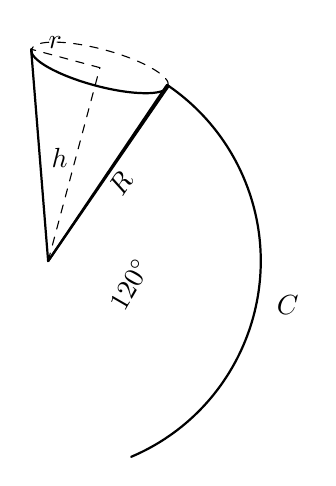
\begin{tikzpicture}[scale=0.9,line cap=round]
  % 圆锥（锥顶与扇形顶点重合）
  \coordinate (V) at (0,0);
  \coordinate (M) at (0.73,2.73);   % 底面椭圆中心（h=2.83，沿 75° 轴）
  \coordinate (P1) at (-0.24,2.99); % 底面椭圆左端
  \coordinate (P2) at (1.70,2.47);  % 底面椭圆右端（与扇形上半径共线）
  \draw[thick] (V)--(P1);
  \draw[thick] (V)--(P2);
  \begin{scope}[shift={(0.73,2.73)},rotate=-15]
    \draw[dashed] (1,0) arc (0:180:1 and 0.26);   % 底面椭圆后半（虚线）
    \draw[thick] (-1,0) arc (180:360:1 and 0.26); % 底面椭圆前半（实线）
\end{scope}
  % 高 h 与底面半径 r（虚线）
  \draw[dashed] (V)--(M);
  \node at (0.16,1.45) {$h$};
  \draw[dashed] (M)--(P1);
  \node at (0.10,3.08) {$r$};
  % 扇形（上半径与圆锥母线 V-P2 重合，标 R；下半径向右下，标弧长记号 C）
  \draw[thick] (V)--(56:3);
  \draw[thick] (-67:3) arc[start angle=-67, end angle=56, radius=3];
  \node[rotate=56] at (1.02,1.10) {$R$};
  \node[rotate=60] at (1.15,-0.32) {$120^\circ$};
  \node at (3.38,-0.62) {$C$};
\end{tikzpicture}
\end{center}
\nopagebreak[4]
\Needspace{0.4\textheight}
\end{question}
\begin{question}
\gkti{3}如图，$AD\text{、}BD$ 分别为 $\triangle ABC$ 的角平分线，延长 $AD$ 交 $\triangle ABC$ 的外接园于 $E$，连接 $BE$，求证：$BE=DE$。

\begin{gktip}
原源 PDF 第 3 页附有 $\triangle ABC$ 外接园示意图，弧上标有记号 1、2、3、4；LaTeX 版按源图重绘。
\end{gktip}
\nopagebreak[4]
\begin{center}% 1977 年四川卷第三题：△ABC 的外接园，AD、BD 为角平分线，
% AD 延长交园于 E，BD 延长交园于 F，求证 BE=DE；
% 弧上记号：1（弧BE）、2（弧EC）、3（弧CF）、4（弧AF）（按源卷第 3 页布局）
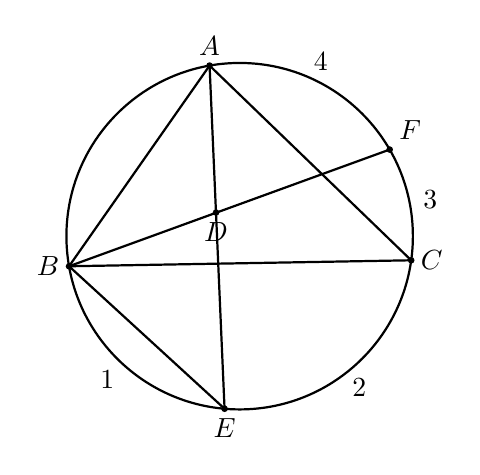
\begin{tikzpicture}[scale=1.0]
  \coordinate (A) at (100:2.2);
  \coordinate (F) at (30:2.2);
  \coordinate (C) at (-8:2.2);
  \coordinate (E) at (265:2.2);
  \coordinate (B) at (190:2.2);
  \coordinate (D) at (-0.30,0.30); % AE 与 BF 的交点
  \draw[thick] (0,0) circle (2.2);
  \draw[thick] (A)--(B)--(C)--cycle;
  \draw[thick] (A)--(E);
  \draw[thick] (B)--(F);
  \draw[thick] (B)--(E);
  \fill (A) circle (1.2pt) node[above] {$A$};
  \fill (B) circle (1.2pt) node[left] {$B$};
  \fill (C) circle (1.2pt) node[right] {$C$};
  \fill (D) circle (1.2pt) node[below] {$D$};
  \fill (E) circle (1.2pt) node[below] {$E$};
  \fill (F) circle (1.2pt) node[above right] {$F$};
  \node at (-1.68,-1.82) {$1$};
  \node at (1.52,-1.92) {$2$};
  \node at (2.42,0.46) {$3$};
  \node at (1.03,2.22) {$4$};
\end{tikzpicture}
\end{center}
\nopagebreak[4]
\end{question}
\begin{question}
\gkti{4}\textbf{（16 分）} 顺次连接 $A(-2,4)$，$B(2,2)$，$C(4,0)$ 得 $\triangle ABC$，写出 $BC$ 边上的高所在的直线方程，并计算 $\triangle ABC$ 的面积。

\end{question}
\begin{question}
\gkti{5}\textbf{（16 分）} 如图，在梯形 $ABCD$ 中，$a:b:c:d=1:3:1:2$。求在梯形 $ABCD$ 中，$\cos\alpha$，$\sin\alpha$ 和 $\sin\beta$ 的值。

\end{question}
\begin{question}
\gkti{6}分别在三个平面直角坐标上作出下列方程的图形。

\begin{gktip}
\textbf{题号说明}：原卷本题三个小题印作“1．”“2．”“3．”，本卷按小问格式重排为（1）（2）（3），未增删题干。
\end{gktip}

（1） $(x+2)(y-1)=0$；

（2） $(x+2)^2+(y-1)^2=0$；

（3） $(x+2)^2-(y-1)^2=0$。

\begin{gktip}
\textbf{参考题}
\textbf{源卷说明}：参考题供超过高中水平的高中生做，考生在答完正题后，若有余力应做此题，在总分之外加分，如作正确解答，正题和参考题总分为 120 分。
\textbf{题号说明}：参考题两题的小题原卷印作“1．”“2．”“3．”，本卷按小问格式重排为（1）（2）（3），未增删题干。
\end{gktip}

\textbf{参考题 1．}

（1） 求函数 $f(x)=\frac14x^4-x^3-2x^2+3$ 的极值。（4 分）

\Needspace{5\baselineskip}
（2） 计算

\nopagebreak[4]
\[
\int\left(\frac{1}{\sqrt{1-x^2}}-\frac{x^2}{\sqrt{4-x^2}}\right)dx.
\]

（4 分）

\Needspace{5\baselineskip}
（3） 计算

\nopagebreak[4]
\[
\iint\limits_{(D)}(1+y^2)\,dx\,dy,
\]

其中 $(D)$ 是 $y=x^2$，$x=y^2$ 所围成的区域。（4 分）

\textbf{参考题 2．} 求下列方程的通解：

（1） $x\,dy-2y\,dx=3x^2\,dx$；

（2） $y''-2y'+y=\cos x$。

\end{question}